\subsection{Diseño de la Base del Manipulador}

La base del manipulador constituye la interfaz mecánica entre el robot PhantomX Pincher y la plataforma del kit. Su diseño se fundamentó en la preservación de características funcionales de la base original, incorporando mejoras estructurales y adaptaciones específicas para el nuevo sistema.

\subsubsection{Análisis de la Base Original}

La base original del robot PhantomX Pincher AX-12 (Figura \ref{fig:ensambleOldBaseArm}) sirvió como referencia para el diseño, proporcionando información valiosa sobre dimensiones, sistemas de fijación y requisitos operativos.

\begin{figure}[H]
    \centering
    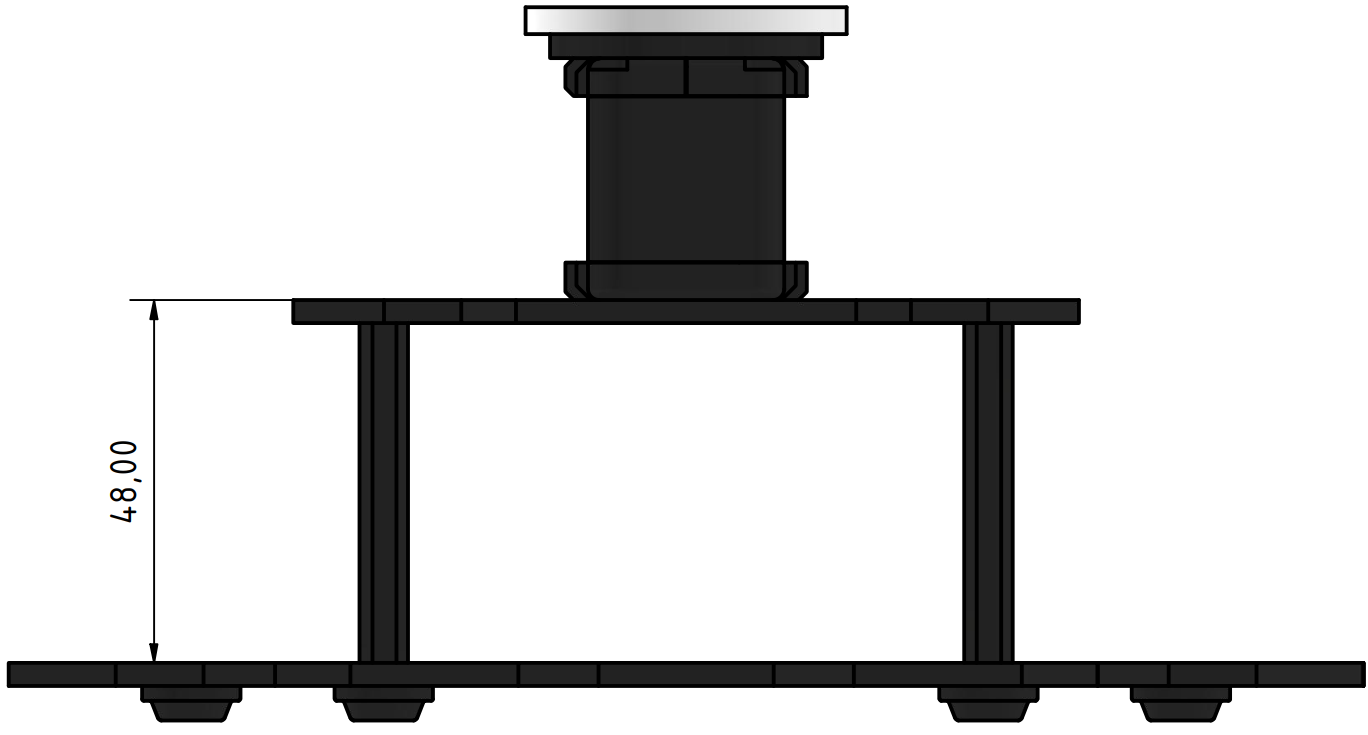
\includegraphics[width=0.6\textwidth]{06disenoConceptual/img/oldArm/medidaBaseArmOld.png}
    \caption{Base original del robot PhantomX Pincher AX-12. (1) Base superior de acrílico que soporta el servomotor principal, (2) Base inferior de acrílico para fijación a superficies, (3) Cuatro espaciadores hexagonales de nylon M3, (4) Manipulador PhantomX Pincher. Se observan las ranuras laterales para paso de cableado.}
    \label{fig:ensambleOldBaseArm}
\end{figure}

\begin{table}[H]
\centering
\caption{Componentes de la base original del PhantomX Pincher AX-12}
\label{tab:base_original}
\small
\begin{tabular}{|c|l|c|l|}
\hline
\textbf{\#} & \textbf{Componente} & \textbf{Cant.} & \textbf{Material} \\
\hline
1 & Base superior de manipulador & 1 & Acrílico \\
2 & Base inferior de manipulador & 1 & Acrílico \\
3 & Espaciador hexagonal de nylon M3 & 4 & Nylon \\
4 & Manipulador & 1 & --- \\
\hline
\end{tabular}
\end{table}

La altura de la base original es de 48 mm (Figura \ref{fig:medidaBaseArmOld}), dimensión que se conservó en el diseño final para mantener la compatibilidad cinemática con los algoritmos de control existentes.

\begin{figure}[H]
    \centering
    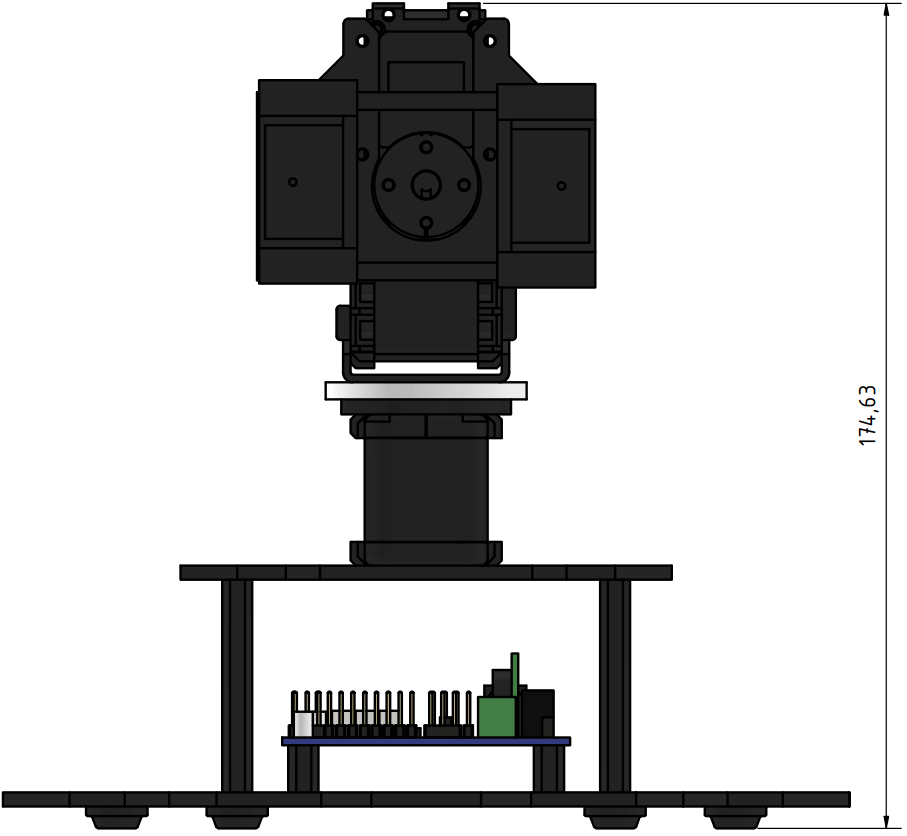
\includegraphics[width=0.5\textwidth]{06disenoConceptual/img/oldArm/medidasPXPAX-12old.png}
    \caption{Vista lateral de la base original mostrando la altura total de 48 mm desde la superficie de montaje hasta la interfaz del manipulador.}
    \label{fig:medidaBaseArmOld}
\end{figure}

\subsubsection{Características Preservadas del Diseño Original}

Del diseño original se conservaron los siguientes elementos funcionales:

\begin{itemize}
    \item \textbf{Sistema de espaciadores hexagonales}: Se mantiene el uso de cuatro espaciadores M3 para fijación del manipulador, garantizando compatibilidad mecánica
    \item \textbf{Ranuras laterales de cableado}: Se preservan las dos aberturas laterales que permiten el paso de cables desde la zona de electrónica hasta el manipulador
    \item \textbf{Altura estándar}: Se conserva la altura de 48 mm para mantener la compatibilidad con la cinemática del robot
\end{itemize}

\subsubsection{Modificaciones e Innovaciones del Diseño}

El diseño final incorpora mejoras significativas respecto a la base original:

\paragraph{Eliminación de la Base Inferior}

Se suprimió la placa inferior de la base original, ya que la plataforma del kit cumple esta función. Esta simplificación reduce:
\begin{itemize}
    \item Número de componentes del sistema
    \item Costo de fabricación
    \item Peso total del conjunto
    \item Complejidad de ensamblaje
\end{itemize}

\paragraph{Integración con Sistema de Vacío}

Se diseñó una cavidad semicircular en la parte posterior de la base (visible en la Figura \ref{fig:medidasBaseArm}) para alojar la bomba de vacío. Esta integración permite:
\begin{itemize}
    \item Aprovechamiento óptimo del espacio disponible
    \item Proximidad entre bomba de vacío y manipulador, minimizando longitud de mangueras
    \item Protección parcial de la bomba dentro del volumen de la base
\end{itemize}

\begin{figure}[H]
    \centering
    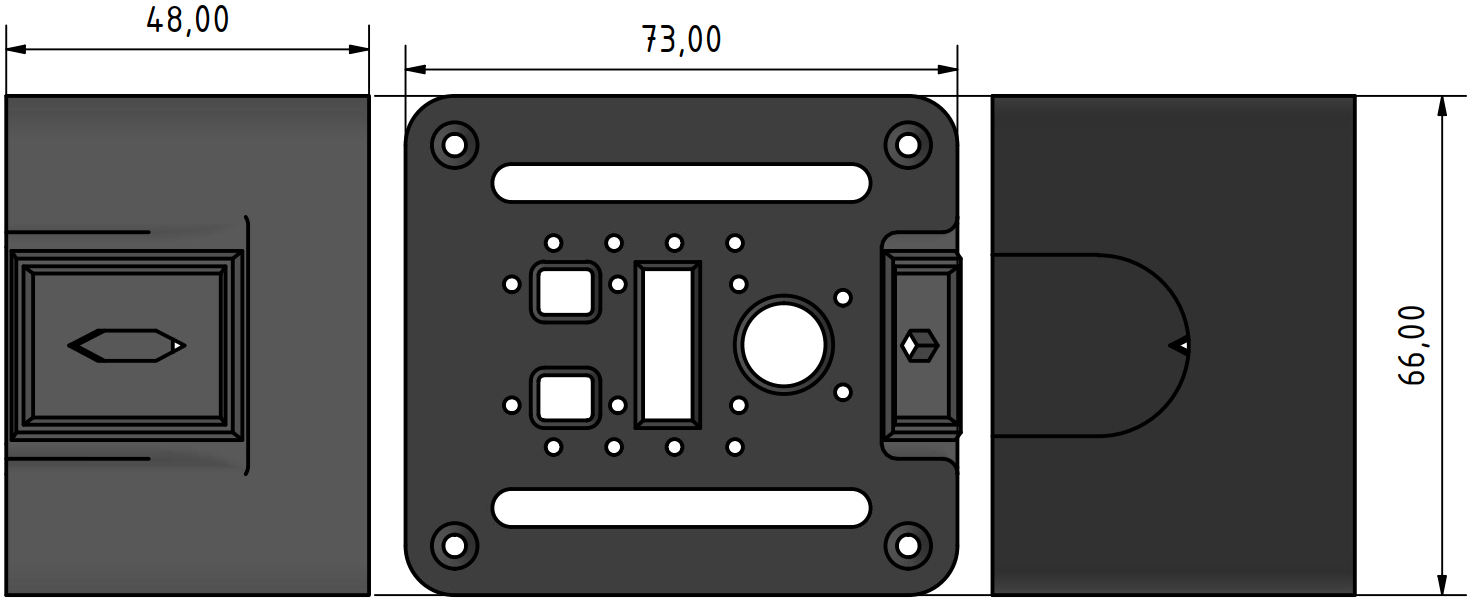
\includegraphics[width=0.75\textwidth]{06disenoConceptual/img/baseArm/medidasBaseArm.png}
    \caption{Vista superior de la base del manipulador con dimensiones principales. Dimensiones exteriores: 73 mm × 66 mm. Se observan: cavidad semicircular posterior de 48 mm de diámetro para alojamiento de bomba de vacío, ranuras laterales de cableado, patrón de montaje para espaciadores hexagonales M3, y diversas perforaciones para paso de cables y ventilación.}
    \label{fig:medidasBaseArm}
\end{figure}

\paragraph{Sistema de Identificación}

Dado que se fabricarán siete kits completos, se incorporó un sistema de identificación mediante una placa plástica intercambiable montada en el frente de la base. Esta ubicación frontal fue seleccionada por:
\begin{itemize}
    \item Alta visibilidad desde cualquier ángulo de aproximación al kit
    \item Facilidad de lectura para usuarios y personal de laboratorio
    \item Posibilidad de reemplazo sin desmontar el manipulador
\end{itemize}

\paragraph{Mejora del Material de Espaciadores}

Se sustituyeron los espaciadores hexagonales de nylon por espaciadores de latón M3 × 30 mm. Esta modificación se fundamentó en la experiencia operativa: durante el desmontaje del manipulador de su base original, varios espaciadores de nylon se fracturaron. El latón ofrece:
\begin{itemize}
    \item Mayor resistencia mecánica a cargas de tracción y compresión
    \item Durabilidad superior frente a ciclos repetidos de montaje/desmontaje
    \item Roscas más resistentes al desgaste
    \item Mejor tolerancia dimensional
\end{itemize}

\paragraph{Soporte Estructural Mejorado}

A diferencia de la base original que se apoyaba únicamente en cuatro puntos (los espaciadores), el diseño final apoya todo su perímetro sobre la plataforma base. Esta configuración proporciona:
\begin{itemize}
    \item Mayor rigidez estructural del conjunto
    \item Distribución más uniforme de cargas operativas
    \item Reducción de vibraciones durante movimientos del manipulador
    \item Estabilidad mejorada para operaciones de alta precisión
\end{itemize}

\subsubsection{Restricciones Dimensionales}

Las dimensiones en planta de la base (73 mm × 66 mm) se determinaron considerando las restricciones espaciales impuestas por el layout de la plataforma (Figura \ref{fig:layout2}). Específicamente, el área ocupada por la base no debe interferir con el cierre de las tapas deslizantes de las canecas adyacentes. Un incremento dimensional de la base invadiría la trayectoria de las tapas, impidiendo el cierre completo de las zonas de depósito.

\subsubsection{Ensamble del Conjunto}

El conjunto completo de la base del manipulador se presenta en la Figura \ref{fig:ensambleBaseArm}.

\begin{figure}[H]
    \centering
    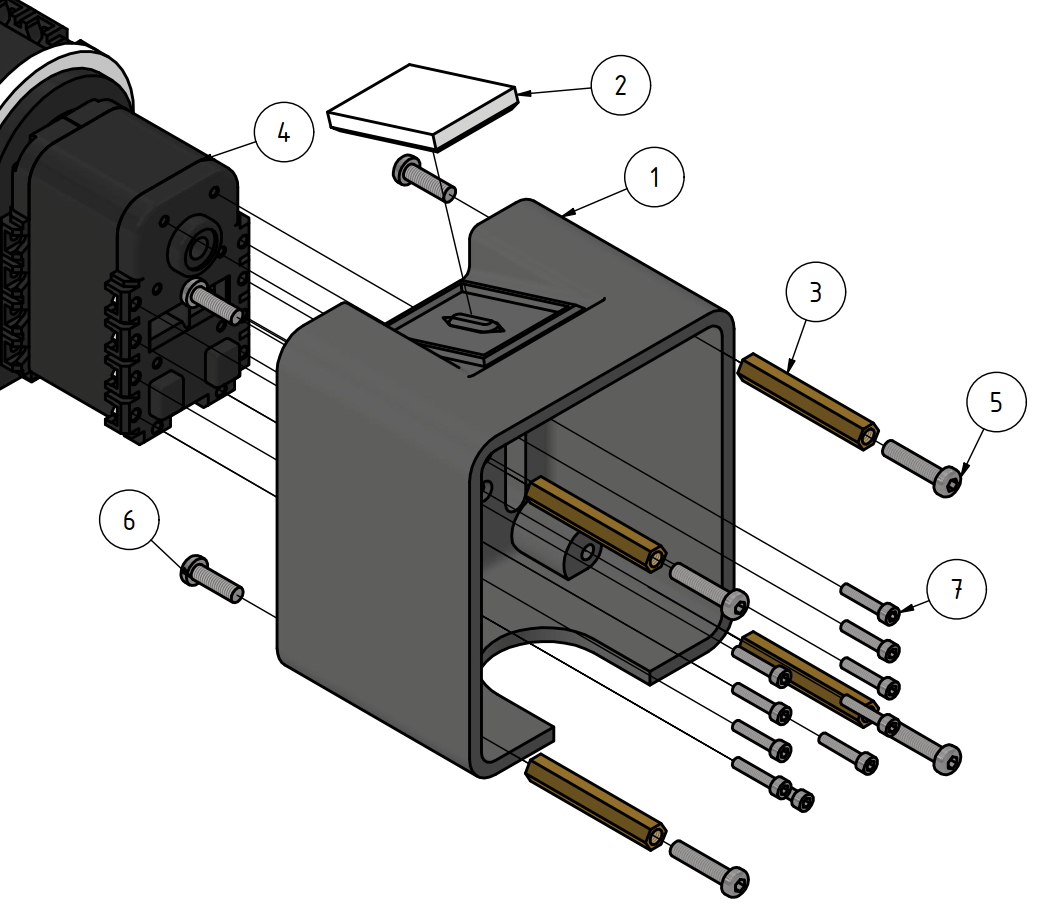
\includegraphics[width=0.85\textwidth]{06disenoConceptual/img/baseArm/ensambleBaseArm.png}
    \caption{Ensamble explosionado de la base del manipulador. (1) Cuerpo de la base fabricado mediante FDM, (2) Placa de identificación numérica intercambiable, (3) Cuatro espaciadores hexagonales de latón M3 × 30 mm, (4) Manipulador PhantomX Pincher, (5) Tornillos M3 × 14 mm para fijación de espaciadores a la base, (6) Tornillos M3 × 10 mm para fijación de la placa identificadora, (7) Tornillos M2 × 10 mm (10 unidades) para fijación del manipulador a los espaciadores.}
    \label{fig:ensambleBaseArm}
\end{figure}

\begin{table}[H]
\centering
\caption{Lista de materiales de la base del manipulador}
\label{tab:bom_base_manipulador}
\small
\begin{tabular}{|c|l|c|l|l|}
\hline
\textbf{\#} & \textbf{Componente} & \textbf{Cant.} & \textbf{Fabricación} & \textbf{Material} \\
\hline
1 & Base de manipulador & 1 & FDM & ABS/PLA \\
2 & Placa de número identificador & 1 & FDM & ABS/PLA \\
3 & Espaciador hexagonal M3 × 30 mm & 4 & Comercial & Latón \\
4 & Manipulador & 1 & --- & --- \\
5 & Tornillo M3 × 14 mm & 4 & Comercial & Acero \\
6 & Tornillo M3 × 10 mm & 4 & Comercial & Acero \\
7 & Tornillo M2 × 10 mm & 10 & Comercial & Acero \\
\hline
\end{tabular}
\end{table}

Los espaciadores hexagonales se fijan a la base mediante tornillos M3 × 14 mm que se enroscan directamente en el latón. El manipulador se monta sobre estos espaciadores utilizando los tornillos M2 × 10 mm originales del robot, reutilizando componentes existentes y reduciendo costos.

El diseño final de la base del manipulador representa una evolución optimizada del concepto original, integrando mejoras estructurales, consideraciones de manufactura, y requisitos específicos del sistema completo del kit educativo.